\documentclass[10pt]{report}

\title{Teknologiprosjekt: Øving 1}
\author{Mathias Mellemstuen}
\date{17.09.20}

\DeclareFixedFont{\ttb}{T1}{txtt}{bx}{n}{10} % for bold
\DeclareFixedFont{\ttm}{T1}{txtt}{m}{n}{10}  % for normal
\usepackage[margin=1in]{geometry}
\usepackage{color}
\usepackage{graphicx}
\usepackage{listings}
\usepackage{wrapfig}
\usepackage{amsmath}

\definecolor{light}{rgb}{0.5, 0.5, 0.5}
\def\lighterText#1{{\color{light}#1}}
\definecolor{deepblue}{rgb}{0,0,0.5}
\definecolor{deepred}{rgb}{0.8,0,0}
\definecolor{deepgreen}{rgb}{0,0.5,0}
\definecolor{grey1}{rgb}{0.5,0.5,0.5}


% Python style for highlighting
\newcommand\pythonstyle{\lstset{
		language=Python,
		basicstyle=\tiny\ttm,
		otherkeywords={self},             % Add keywords here
		keywordstyle=\tiny\ttb\color{deepblue},
		emph={},          % Custom highlighting
		emphstyle=\tiny\color{deepred},    % Custom highlighting style
		stringstyle=\tiny\color{deepgreen}\ttm,
		commentstyle=\tiny\color{grey1}\ttm,
		frame=none,                         % Any extra options here
		showstringspaces=false,            % 
		breaklines=true,
		tabsize=2
}}
% Python environment
\lstnewenvironment{python}[1][] {
	\pythonstyle
	\lstset{#1}
}{}

% Python for external files
\newcommand\pythonexternal[2][]{{
		\pythonstyle
		\lstinputlisting[#1]{#2}}}

% Python for inline
\newcommand\pythoninline[1]{{\pythonstyle\lstinline!#1!}}

\newcommand{\Vi}{\vec{i}}

\begin{document}
\begin{flushright}
\lighterText{Mathias Mellemstuen (17.09.20)}
\end{flushright}
\begin{center}
\section*{Teknologiprosjekt: Øving 1}
\textbf{Robotarium experiment with motion planning and control}
\line(1,0){400}
\end{center}
The undertaken task was to design, simulate, test and implement a simple motion planning and control algorithm. The motion control algorithm should be written in Python and tested on the Robotarium robotics simulator.
Python code can be deployed on a real robot when the code is thoroughly tested with the Robotarium simulator.
The robot should follow a track which resembles the shape of the infinity symbol.
\\\\
\textbf{Creating the Infinity track}\\

The array with all the coordinates could then be two-dimentional and defined like this: 
\begin{python}
    path = [
        [0.0, ...], # Array with x coordinates
        [0.0, ...]  # Array with y coordinates
    ]
\end{python}
The Robatarium API has a function that allows you to plot lines between points. This function can be used to draw the track with the path variable like this: 
\begin{python}
# Plotting a red line between the points in the path. 
def plotTrack():
    r.axes.plot(path[0],path[1],color='red',linewidth = lineWidth)
\end{python}
Since the edges of the infinity symbol is circular, it will also need a way to plot points in a circle:
\begin{python}
# Normalizing a value between min - max
def normalize(min, max, value): 
    return min + (max - min) * value 

# Creating a part of a circle fromRadians -> toRadians
def createCircle(x, y, fromRadians, toRadians, step, normalizeMin, normalizeMax): 
    current = fromRadians
    circle = [[],[]]
    while(current < toRadians):
        circle[0].append(x + normalize(normalizeMin, normalizeMax, math.cos(current)))
        circle[1].append(y + normalize(normalizeMin, normalizeMax, math.sin(current)))
        current += step
return circle
\end{python}
Now it's possible to hardcode the straight lines and then use the \pythoninline{createCircle} function to create the curved part of the infinity symbol, then append everything in the right order to \pythoninline{path}.
The end results after doing this looks like this: 
\begin{figure}[h!]
    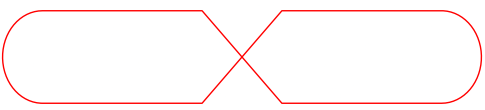
\includegraphics[width=0.5\linewidth]{infinitypicture.png}
\end{figure}
\newpage

\textbf{Motion control algorithm} \\
Since the robot in this case always know it's current (x,y) coordinates and angular rotation at all times,
it would make sense to store the track as an array of (x,y) coordinates and then use trigonometry to find
the distance and angle between the robot and the current waypoint.\\
When the robot is on the current waypoint (n), the current waypoint can then be changed to (n+1).\\
The distance between the robot and the target can be calculated with the pythagoras sentence, $\alpha = \sqrt{\Delta x^{2} + \Delta y^{2}}$.
The equation can be written like this in python: 
\begin{python}
def calculateDistanceBetweenTwoPoints(x1,y1,x2,y2):
    return math.sqrt(math.pow(x2 - x1,2) + math.pow(y2 - y1, 2))
\end{python}
The shortest angle in radians between the robot and the waypoint can be defined like this: $\alpha = atan2(\Delta y, \Delta x)$.
This can be translated to this python function:
\begin{python}
def calculateAngleBetweenPoints(x1,y1,x2,y2):
    deltaX = x2 - x1
    deltaY = y2 - y1
    return math.atan2(deltaY, deltaX)
\end{python}
The
\\\\
\textbf{Results of the simulation} \\
...
\\\\
\textbf{Results of the algorithm deployed on a real robot} \\
...
\end{document}
